\section{Empirical Illustration}
In this section, we illustrate the capabilities of the MINT platform using data from a real experimental study. The empirical illustration is based on \cite{feri2026}, where the authors investigate the interaction between human and machine traders. Specifically, the paper investigates how volume-based information is disseminated in the markets, and whether human participants are able to acquire this information and employ a profitable trading strategy. The authors investigate trading behaviour under different treatments, including treatments where the machine informed traders reach their goal by using only aggressive orders, or scenarios where the machine informed trader uses a mixture of passive and aggressive orders to try and conceal their private information.

The experiments were conducted in June and July 2025, and participants were recruited via the Prolific platform. Each participant, participated in one session, where each session consisted of 6 markets\footnote{The first market was considered as a practise market, and was not taken into account for calculating the final reward.}. For illustration, we present the results from a randomly selected market. In this market, the platform configuration parameters are set as:
\begin{equation*}
\left\{ \tau=3, p_{0} = 100, \sigma=1, \mathbf{g}=[0], |\mathcal{A}_{N}| = 1, \delta = 0.7, \zeta=0.5, |\mathcal{A}_{I}| =1, \beta=0.43, \psi_{I} = \text{False}\right\}
\end{equation*}
The rest follow their default values, as presented in Appendix A, Table \ref{tab:parameters}.

Thus, in this market, a machine informed trader buys 40 shares using only aggressive orders. The human participant acts as a Speculator, and is therefore allowed to post both bid and ask orders, as well as passive and aggressive orders. Their goal is to maximise their profits. In addition, the noise trader posts bid and ask orders with probability 0.5, and sends aggressive orders with probability 0.3. As a result, their impact on expected final price is zero. Instead, the noise trader generates a white-noise effect on the price and exists solely to maintain some level of trading activity, ensure sufficient liquidity in the market.

Thus, the only forces that can shift the price are the trades executed by the machine informed trader and the human participant.
\subsection{Trading behaviour}
Following the above, Figure \ref{fig:empirical_midprice} shows how the market price evolved over the three minute trading activity. Specifically, Panel (a) shows the midprice evolution and Panel (b) illustrates the best bid price $\max(\mathbf{B}_t)$, the best ask price $\min(\mathbf{A}_t)$, as well as the informed trades. 

It is clear that the presence of the informed trader had a profound effect on the market, shifting the midprice by approximately 10 $\sigma$. As shown in Panel (b) of Figure \ref{fig:empirical_midprice}, the informed trader relied exclusively on aggressive orders, crossing the spread. In doing so, the informed trader effectively moved the market, as their trades depleted liquidity at the best available ask orders and pushed both the bid and the ask price to new higher values. 

Thus, it is evident that the informed trader creates opportunities for employing various profitable strategies, such as buying shares early on and selling them later when both the ask and bid prices have risen significantly.
\begin{figure}[!htbp]
    \centering
    \subfloat[\centering Midprice]{{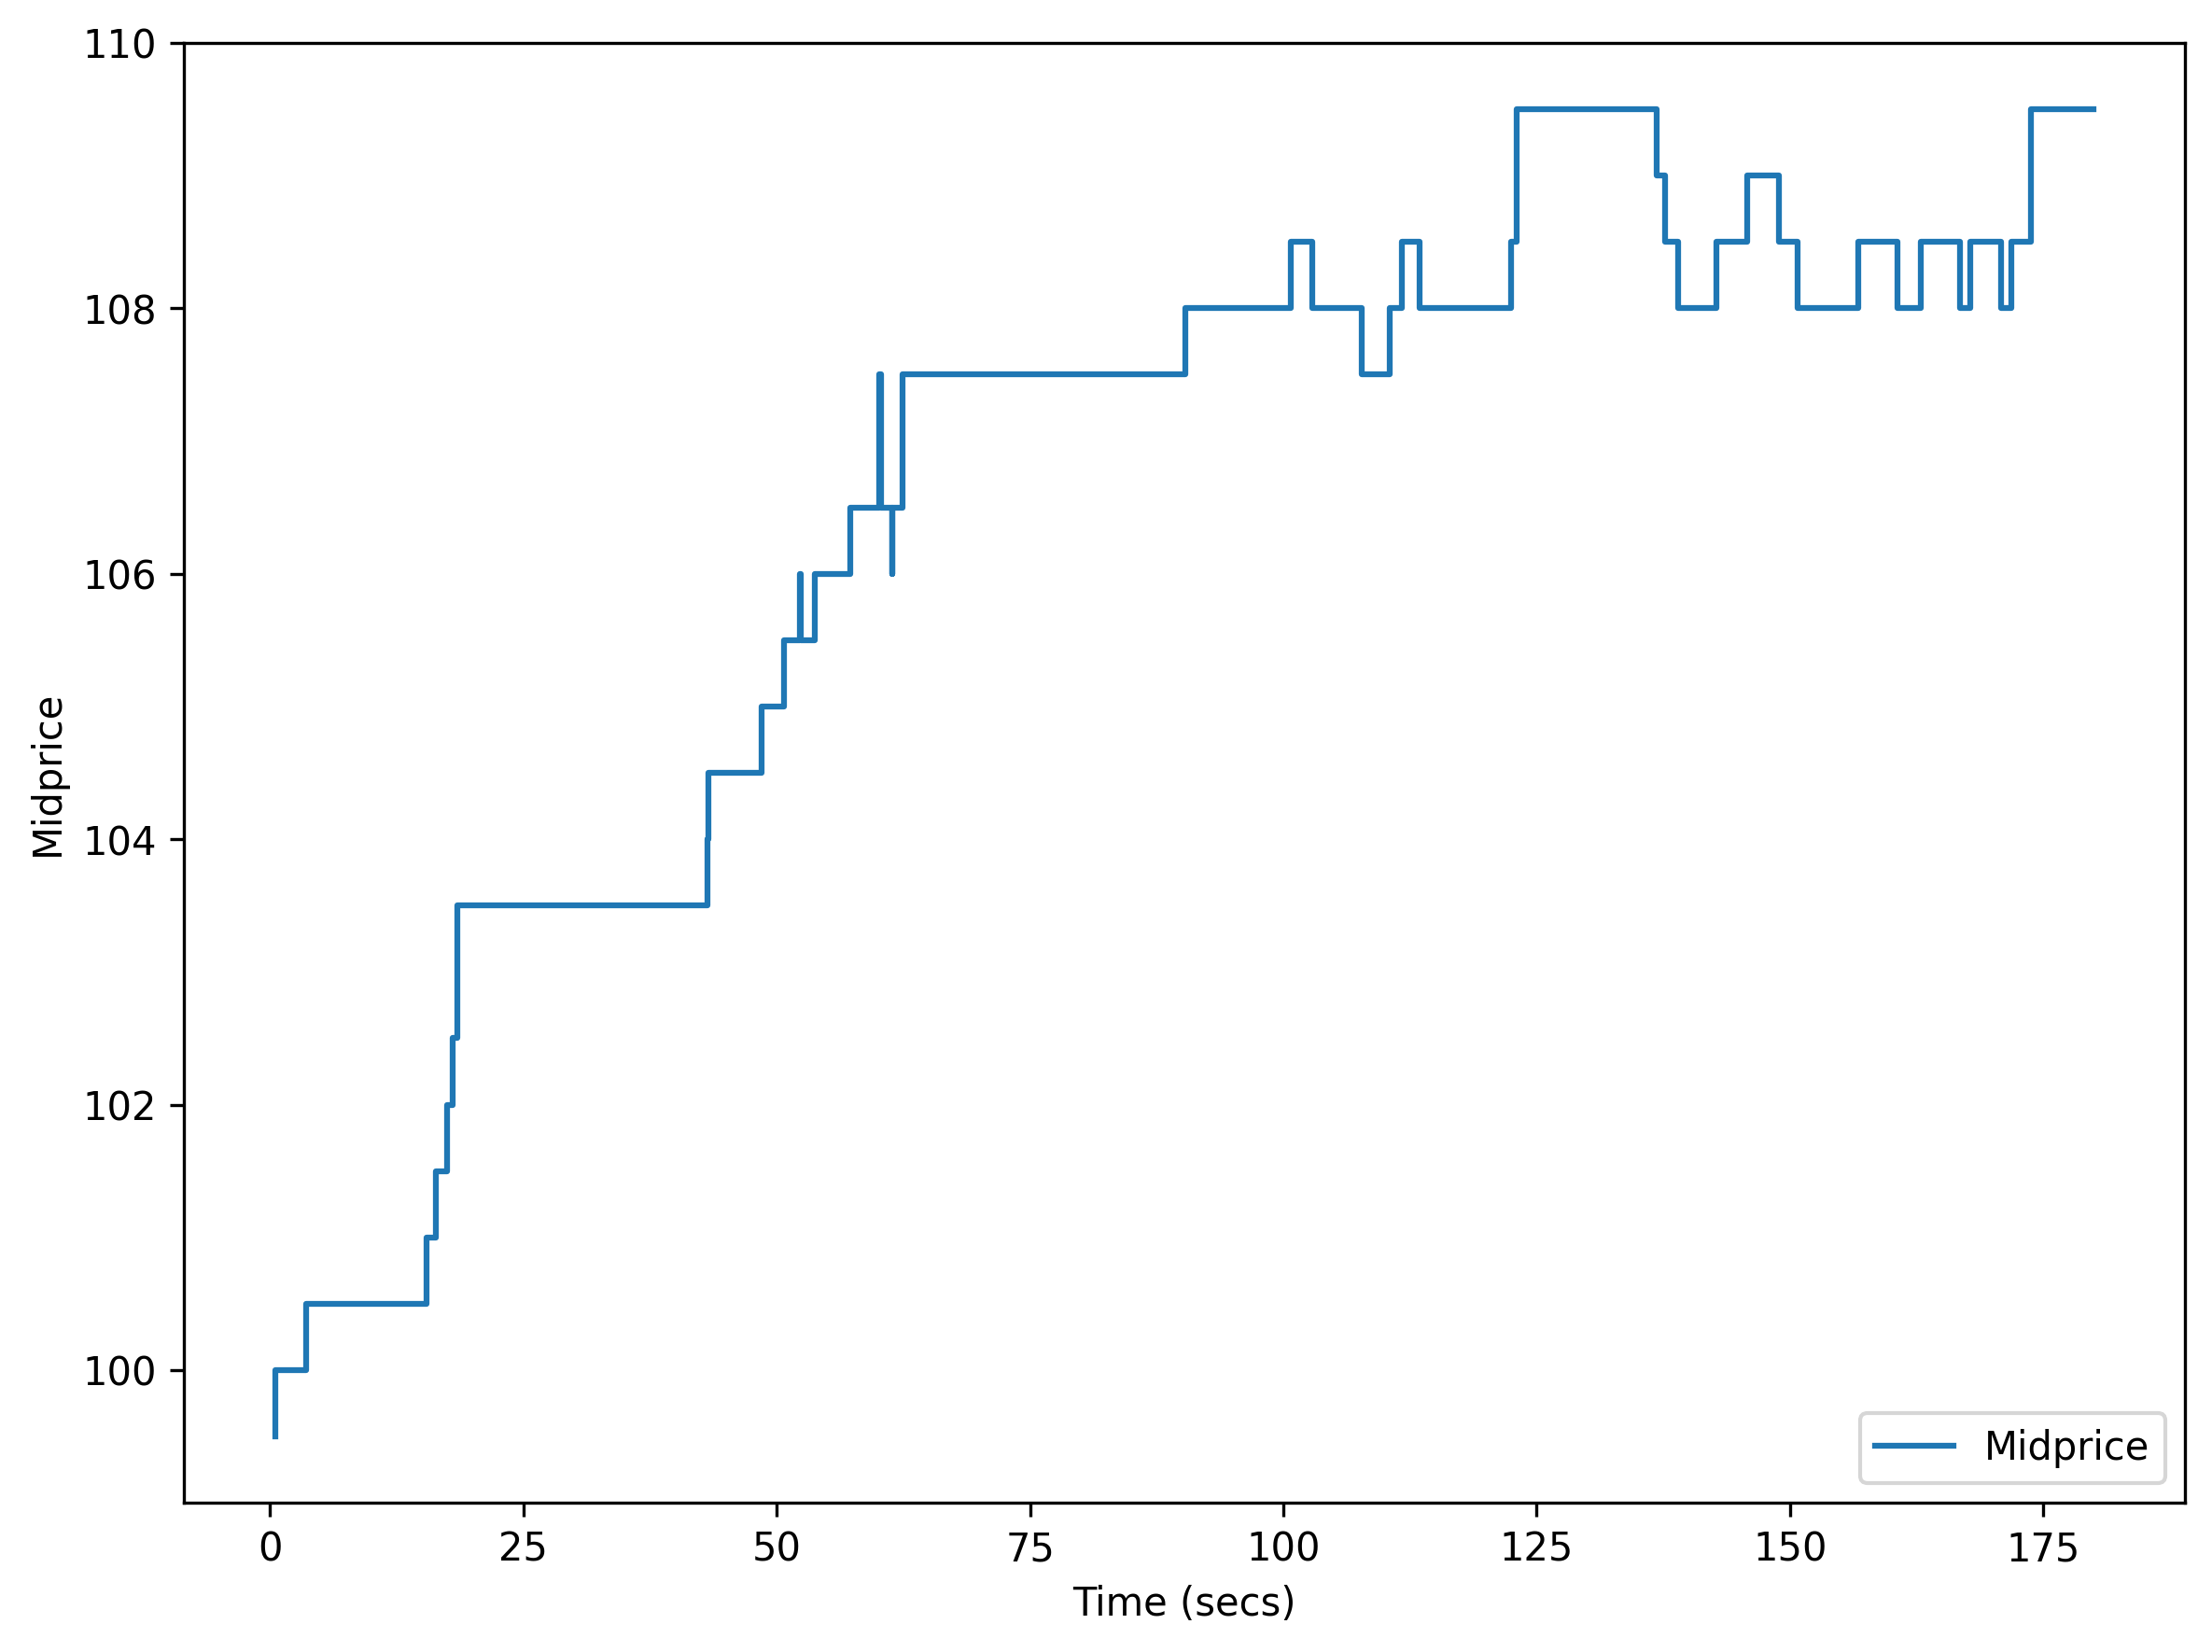
\includegraphics[scale=0.35]{figs/40_midprice.png} }}
    \qquad
    \subfloat[\centering Informed Trades]{{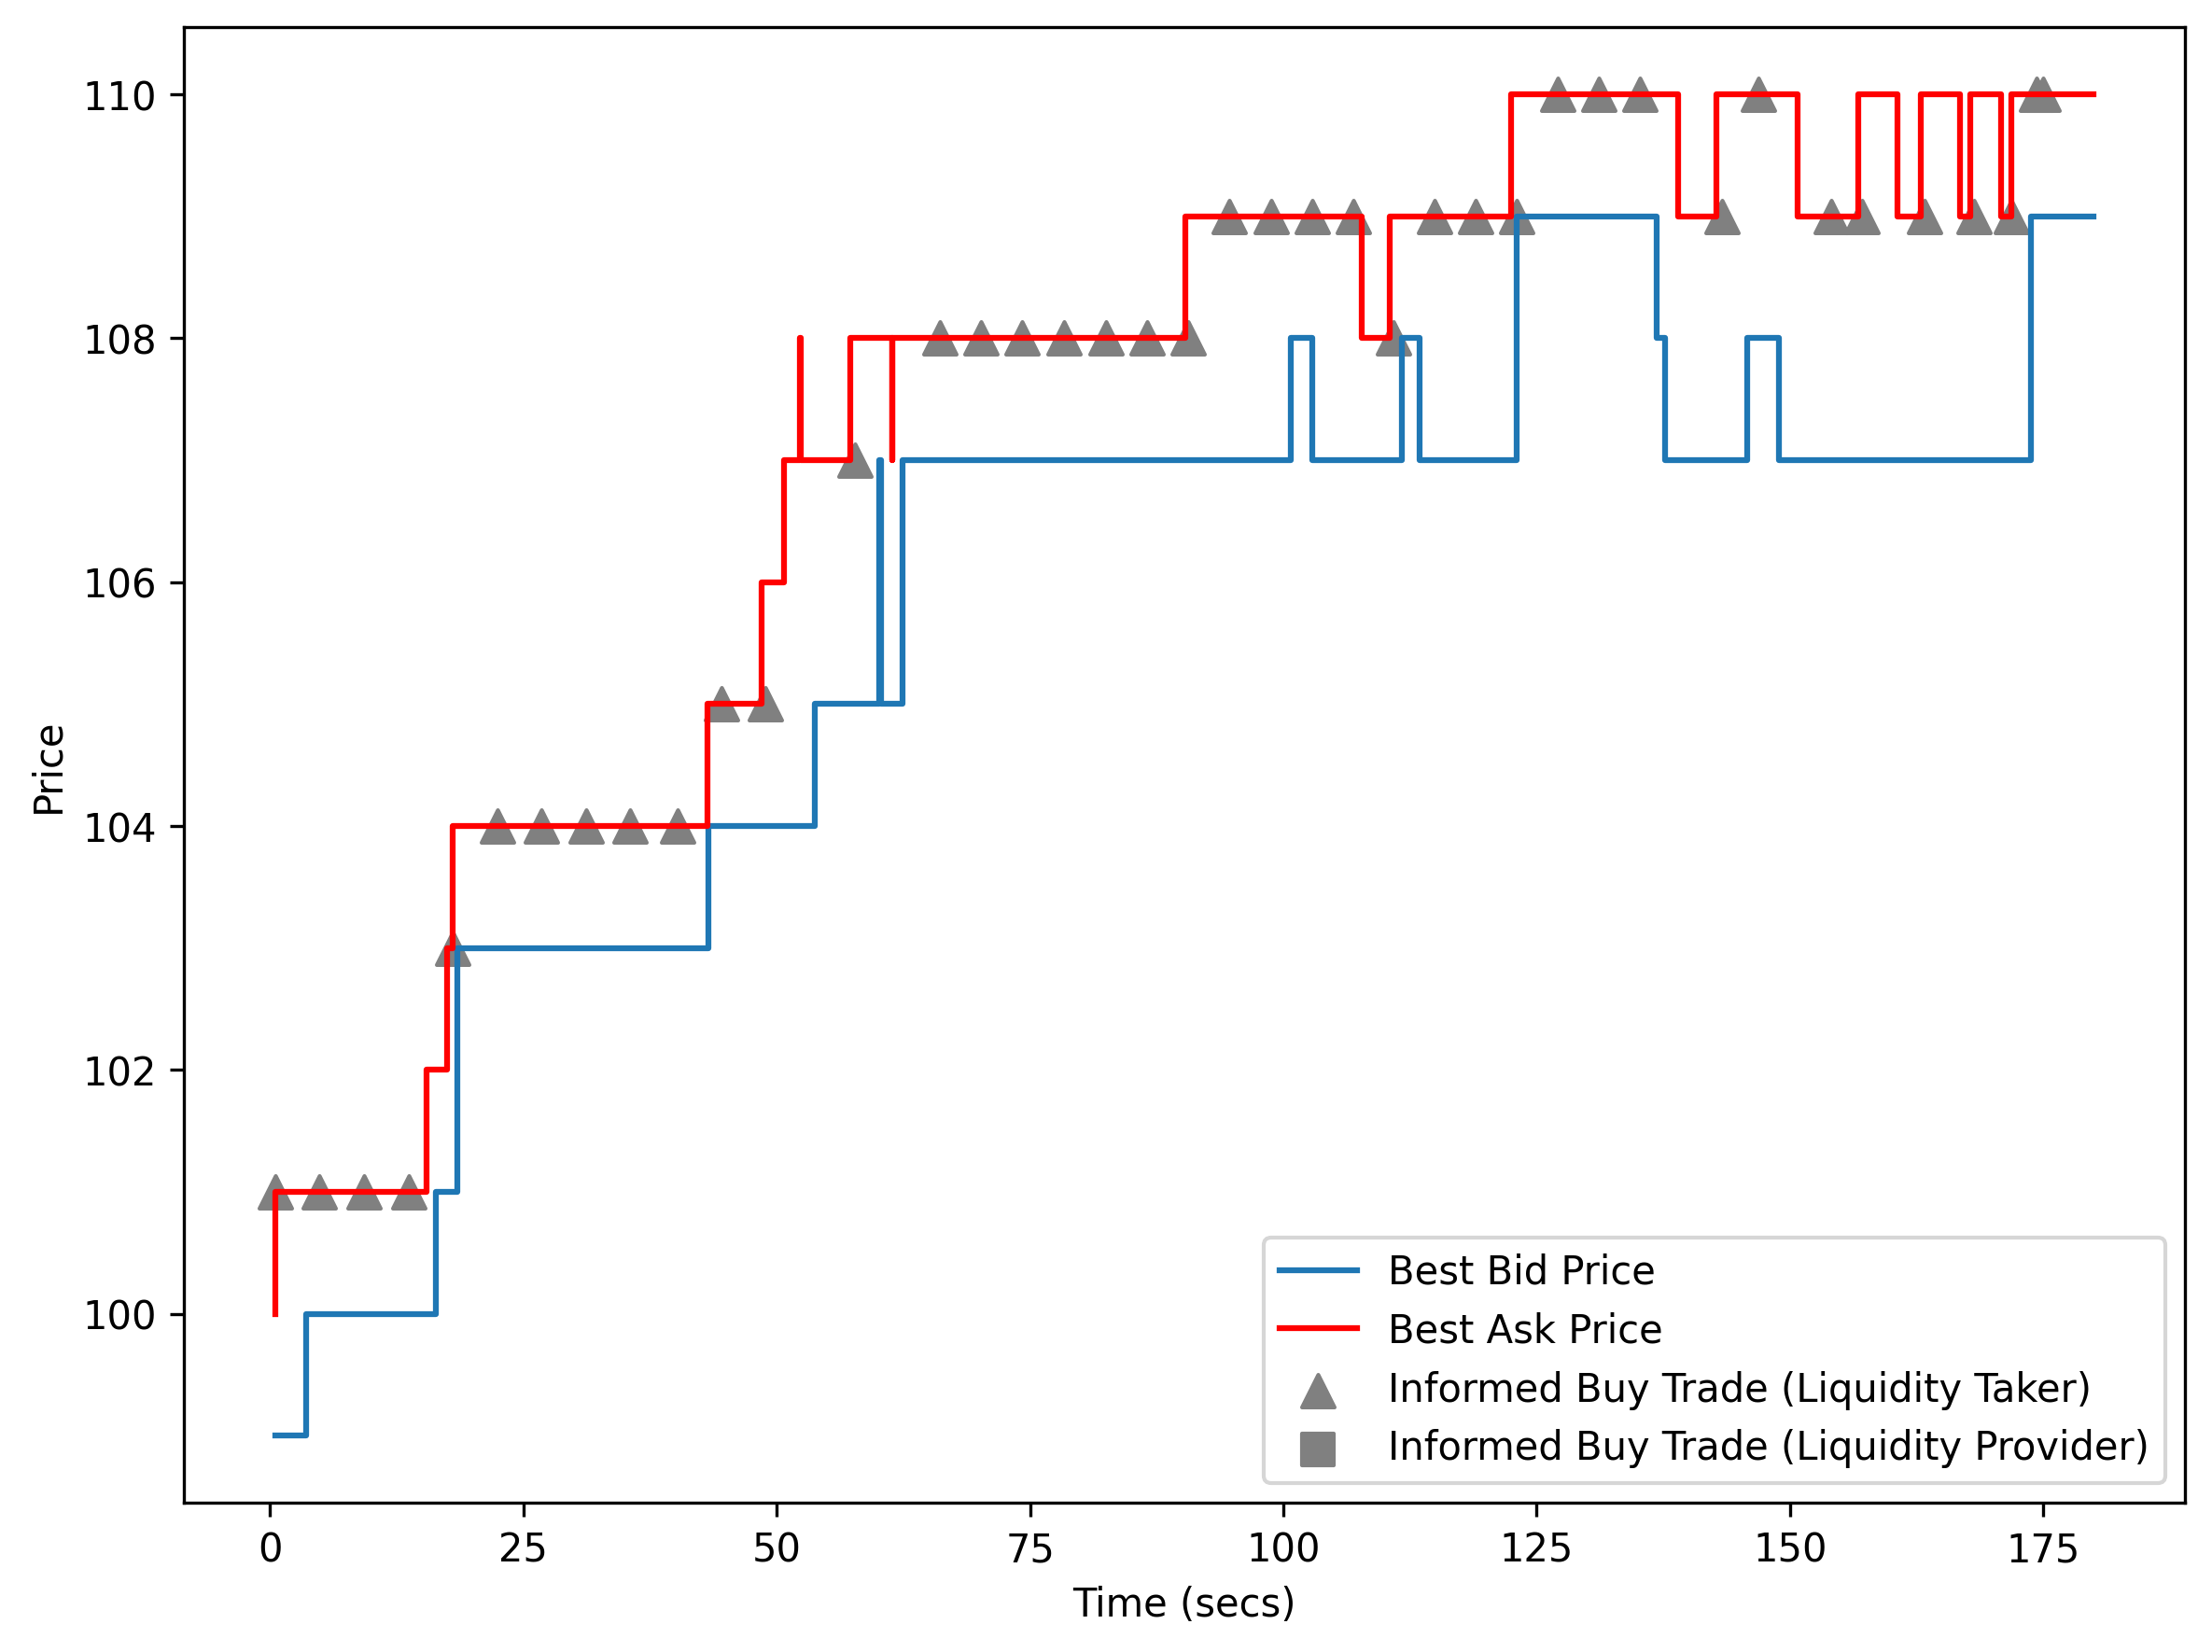
\includegraphics[scale=0.35]{figs/40_informed_trades.png} }}
    \caption{Midprice Evolution and Informed Trading}
    \label{fig:empirical_midprice}
\end{figure}

Next, we analyse the trading behaviour of the human participant. Figure \ref{fig:human_trading_activity} illustrates the trading activity of the participant, as well with their net inventory. Specifically, Panel (a) shows all the limit orders (bid and ask orders) sent by the participant. Panel (b) shows all the human trades classify them as Buy Trades and Sell Trades. Panel (c) depicts the net inventory over the three minutes period.
\begin{figure}[!htbp]
    \centering
    \subfloat[\centering Human Limit Orders]{{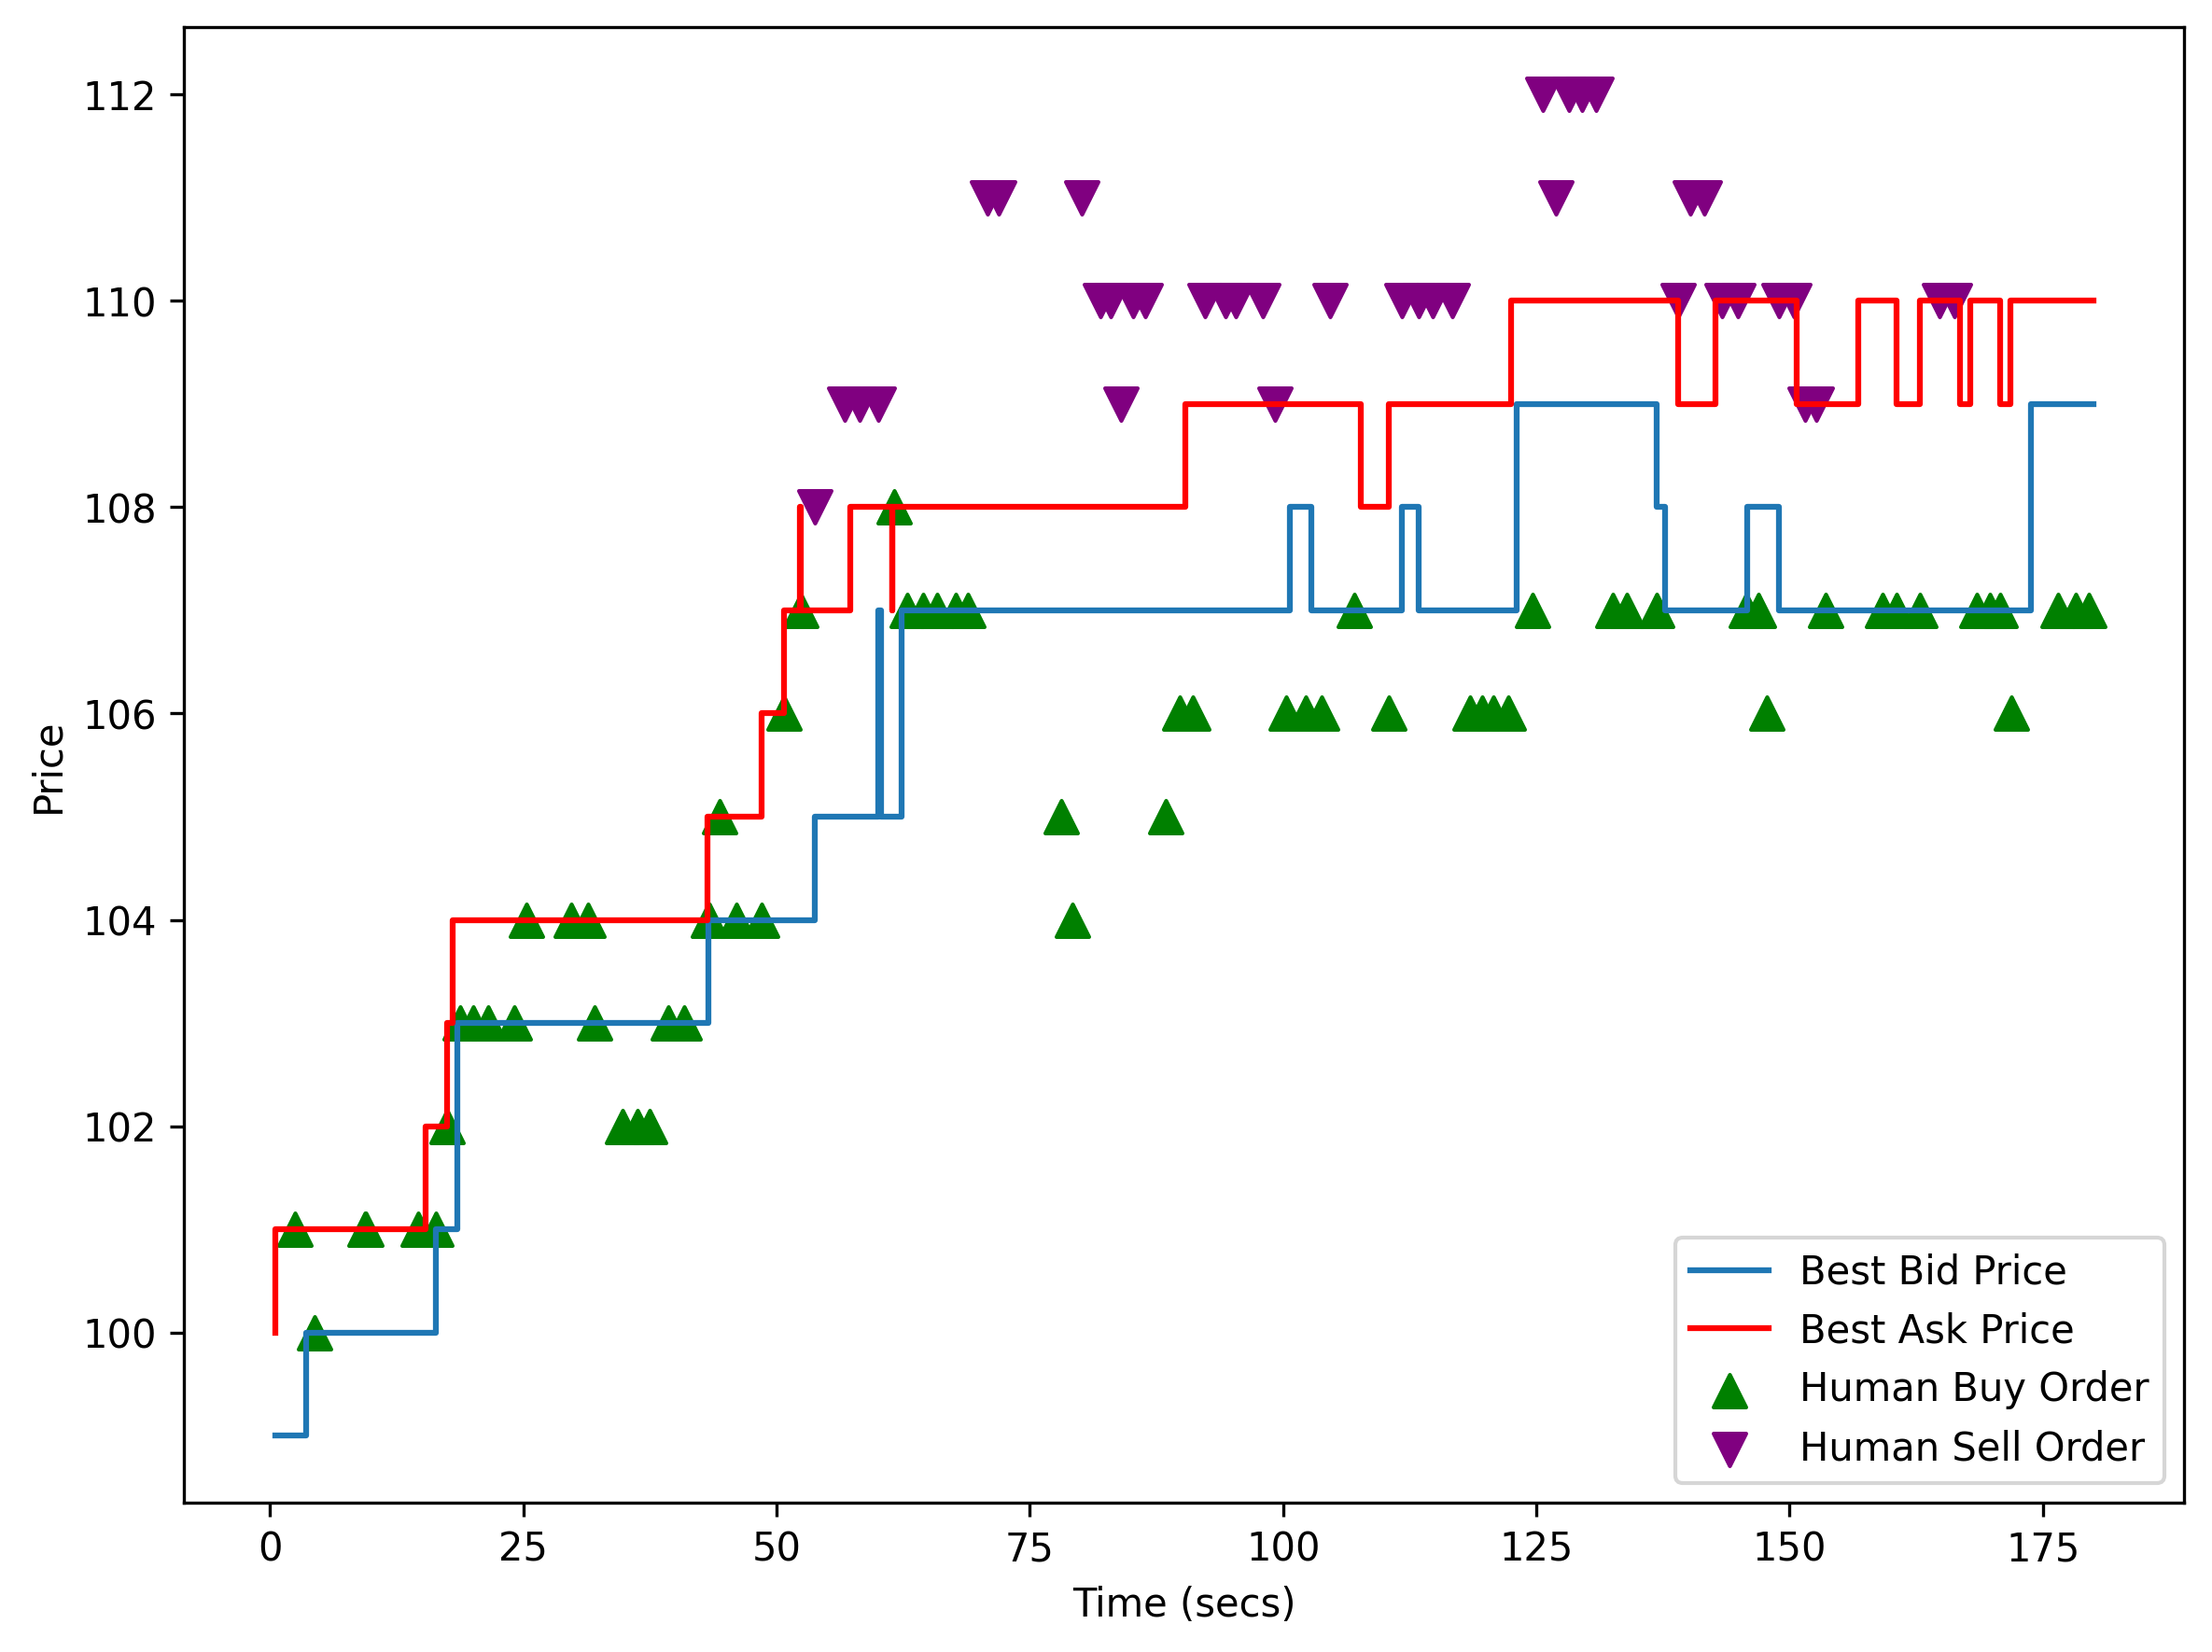
\includegraphics[scale=0.35]{figs/40_orders.png} }}
    \qquad
    \subfloat[\centering Human Trades]{{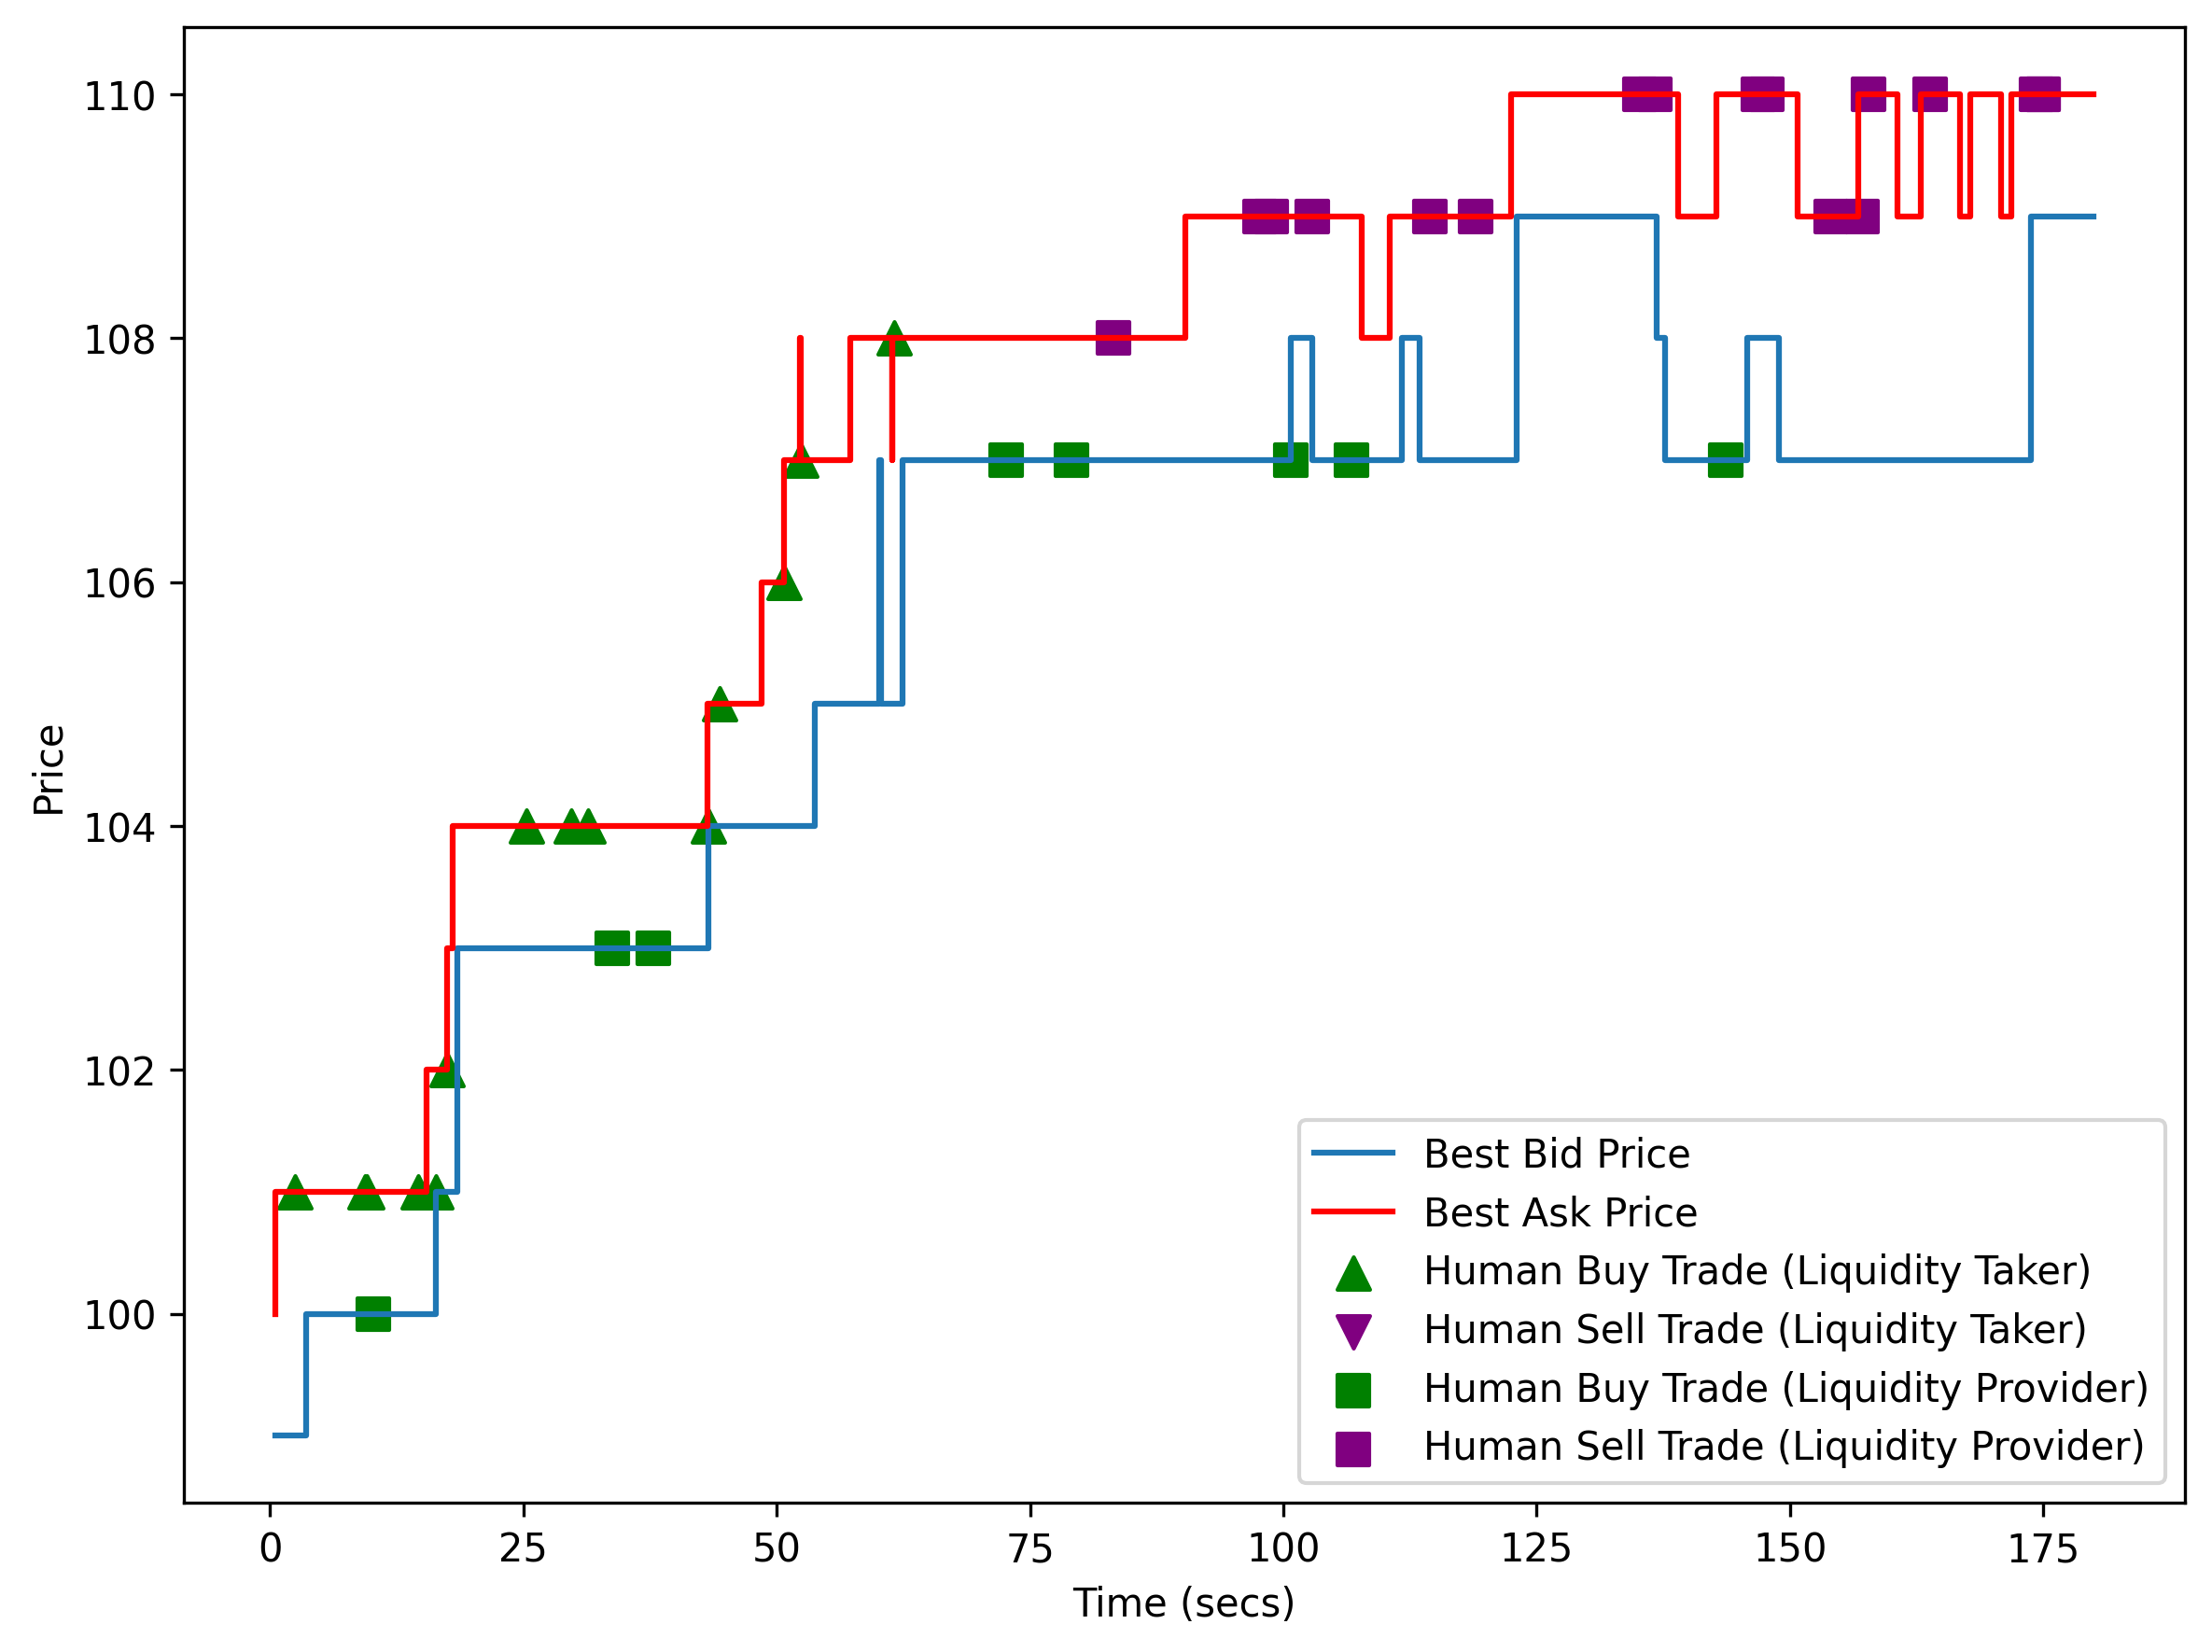
\includegraphics[scale=0.35]{figs/40_trades.png} }}
    \qquad
    \subfloat[\centering Human Net Inventory]{{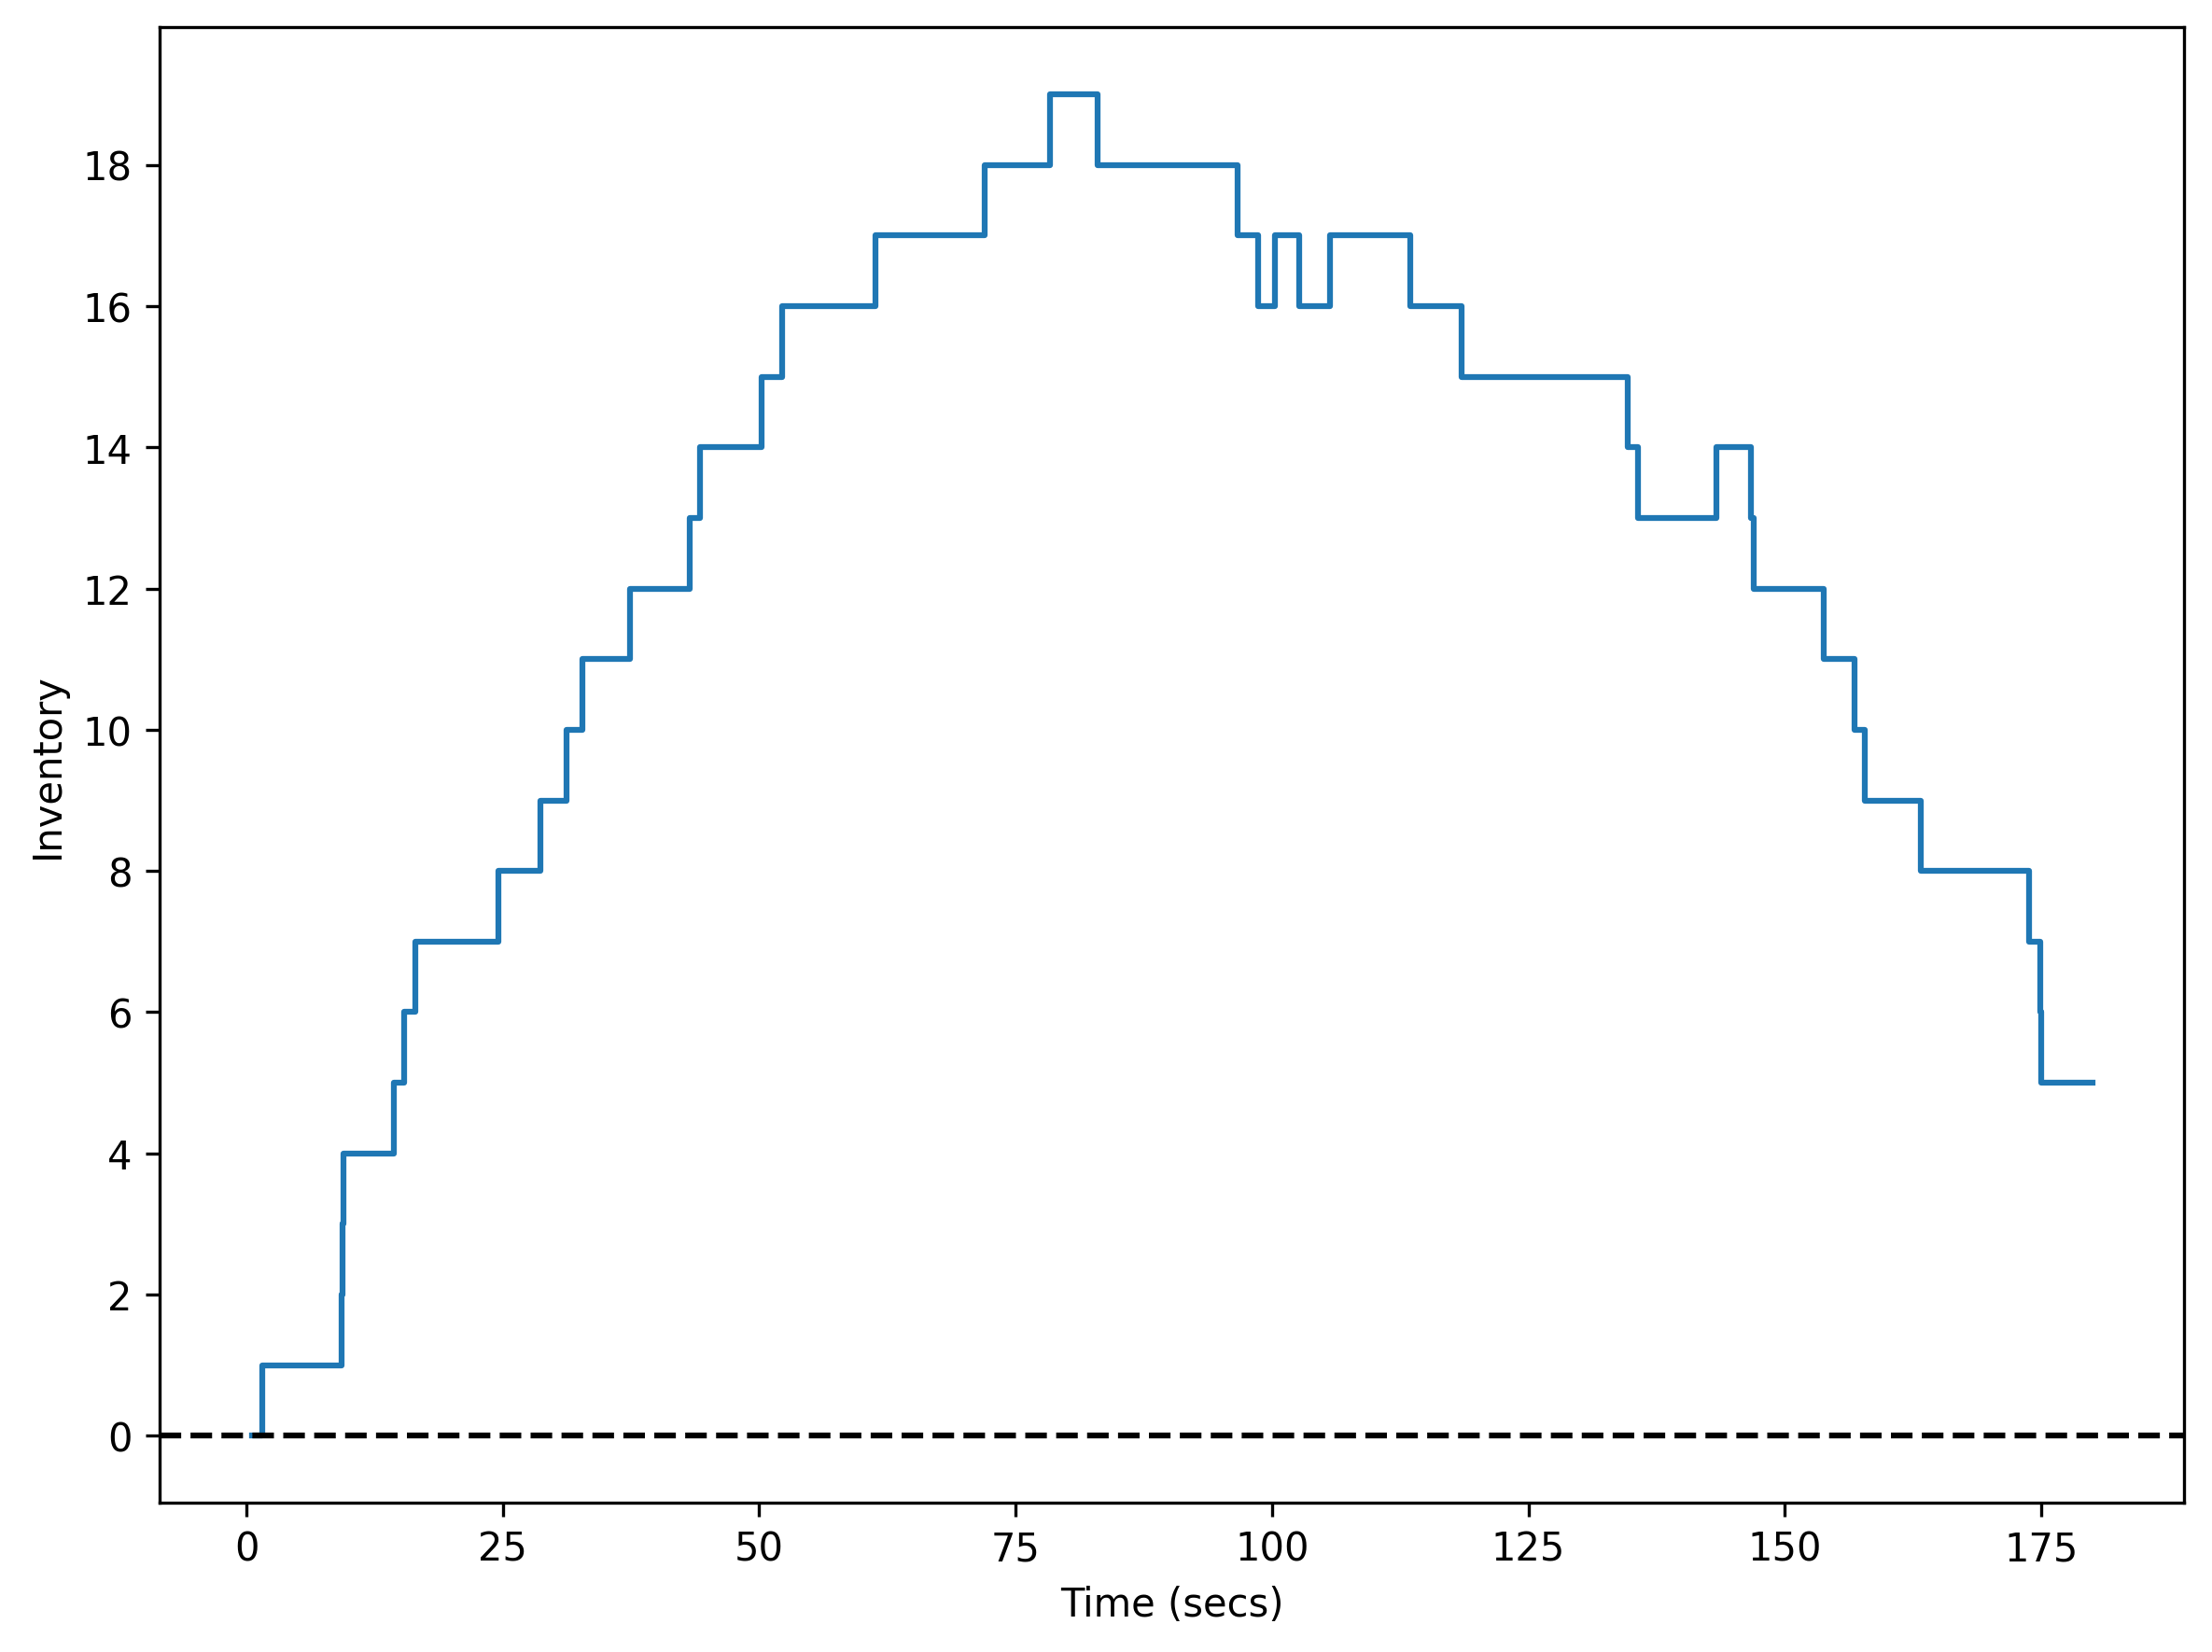
\includegraphics[scale=0.35]{figs/40_inv.png} }}
    \caption{Human Trading Activity}
    \label{fig:human_trading_activity}
\end{figure}

First, from Panel (a) we can see that the human trader employed both passive and aggressive orders, submitting orders at both the top levels and deeper levels of the order book. For instance, while the midprice was around 107-108, the human trader posted ask orders at prices ranging from 110 to 112. This behaviour is consistent  with an expectation of further price increases. Subsequently, Panel (b) presents the human's executed trades, which can be categorised into two two groups: (i) trades initiated through aggressive orders, where the human acted as a ``Liquidity Taker" and (ii) trades initiated by other machine traders (either noise or informed trader) that matched the human's passive orders, meaning that the participant acted as a ``Liquidity Provider". Overall, we can observe that the human participant initially bought shares and, at a later stage, when the price was higher, began to sell them. It is also interesting to note that, in the first stage, all shares were acquired mostly through aggressive orders, whereas the shares were sold exclusively using passive orders. Panel (c), illustrates how the net inventory evolved over the three minute trading activity. We can see, that during the first 90 seconds, the human increased the net inventory by buying 19 shares. After that, the net inventory decreased to 5, a trend that is consistent with the trading behaviour depicted in Panel (b).

Last, Table \ref{tab:empirical_human_trades} summarises the human's trades shown in Figure (\ref{fig:human_trading_activity}), Panel (b). We can see that the $VWAP_{buy} = 104.09$ and the $VWAP_{buy} = 107.32$ , indicating that the participant managed to deploy a profitable strategy. Here, we want to highlight that the last 5 orders at the Sell Trades column (highlighted in red) correspond to the automated platform's orders, which were executed to balance the net inventory\footnote{These trades are executed offline, and their solely purpose is to penalise the unbalanced inventory and adjust the human's reward.}. Interestingly, even thought the participant din't manage to exit the market with a balanced net inventory, in this specific market, the penalisation of the platform, didn't produce negative profitability, and such, the participant managed to make a $PnL = 71$. However, it is important to highlight that the last 5 shares, were executed at the initial midprice $p_{mid,0} = 100$, though the human could have sold them even using aggressive orders, at price $\max(\mathbf{B}_{\tau}) = 109$ achieving an additional profit of approximately 45 Liras.
\begin{table}[!htbp]
\centering
\caption{Summary of Human Buy and Sell Trades}
\label{tab:empirical_human_trades}
\begin{tabular}{cc|cc}
\toprule
\multicolumn{2}{c|}{Buy Trades} & \multicolumn{2}{c}{Sell Trades}\\
Quantity & Price  & Quantity & Price  \\
\hline
1 & 100 & 1 & 108\\
5 & 101 & 7 & 109\\
1 & 102  & 9 & 110\\
2 & 103  & \textcolor{red}{5} & \textcolor{red}{100}\\
4 & 104 \\
1 & 105 \\
1 & 106 \\
6 & 107 \\
1 & 108 \\
\hline
Num. Trades & 22 & Num. Trades & 22  \\
Total Spent & 2290 & Total Received & 2361\\
VWAP & 104.09 & VWAP & 107.32  \\
\bottomrule
\end{tabular}
\end{table}

\subsection{Additional Order Book Metrics}
The MINT platform’s ability to provide replicable and comprehensive Level 3 (L3) quote data not only allows researchers to analyse in detail the trading behaviour of different participants, both human and machine, but also enables the estimation of a wide range of order book metrics that are crucial for understanding market and order book dynamics. Specifically, in the high-frequency trading literature (e.g. \cite{cont2014price}, \cite{ait2022}, \cite{cordoni2024consistent}, \cite{jonuzaj2025} among others), researchers are particularly interested in extracting order book and trading features that can shed light on causal mechanisms, for example, whether specific features can induce certain trader behaviours, predict future price movements, or reveal meaningful signals. These features are therefore essential for both understanding the underlying dynamics of financial markets and for identifying signals that can be used to develop profitable trading strategies.

For instance, some of the most common metrics that researchers are interested in, are:
\begin{itemize}
	\item Order Book Imbalance: 
	\begin{equation*}
	OBI^{(k)}_{t} = \frac{TB^{(k)}_{t} - TA^{(k)}_{t}}{TB^{(k)}_{t}+TA^{(k)}_{t}}
	\end{equation*}
	where $TB^{(k)}_{t}$ and  $TA^{(k)}_{t}$ denote the total number of bid and ask orders, respectively, at the top 	$k$ levels. The $OBI^{(k)}_{t} \in [-1,1]$ and reflects relative imbalance. Apparently, values greater than zero, 	denote that there is a demand pressure, and therefore, one could expect that the price could increase. On the 	other hand, values less than zero, reflect that the market is under selling pressure.
	\item Order Flow Imbalance (OFI):
	\begin{equation*}
	OFI_{t,t-j} = \frac{OFB_{t,t-j} - OFA_{t,t-j}}{OFB_{t,t-j}+OFB_{t,t-j}}
	\end{equation*}
	where $OFB_{t,t-j}$ and $OFA_{t,t-j}$  denotes the order flow of bid and ask orders (passive and aggresive), 	respectively, between the time periods $t-j$ and $t$.
	\item Trade Flow Imbalance (TFI):
\end{itemize}

\begin{figure}[!htbp]
    \centering
    \subfloat[\centering Order Book Imbalance]{{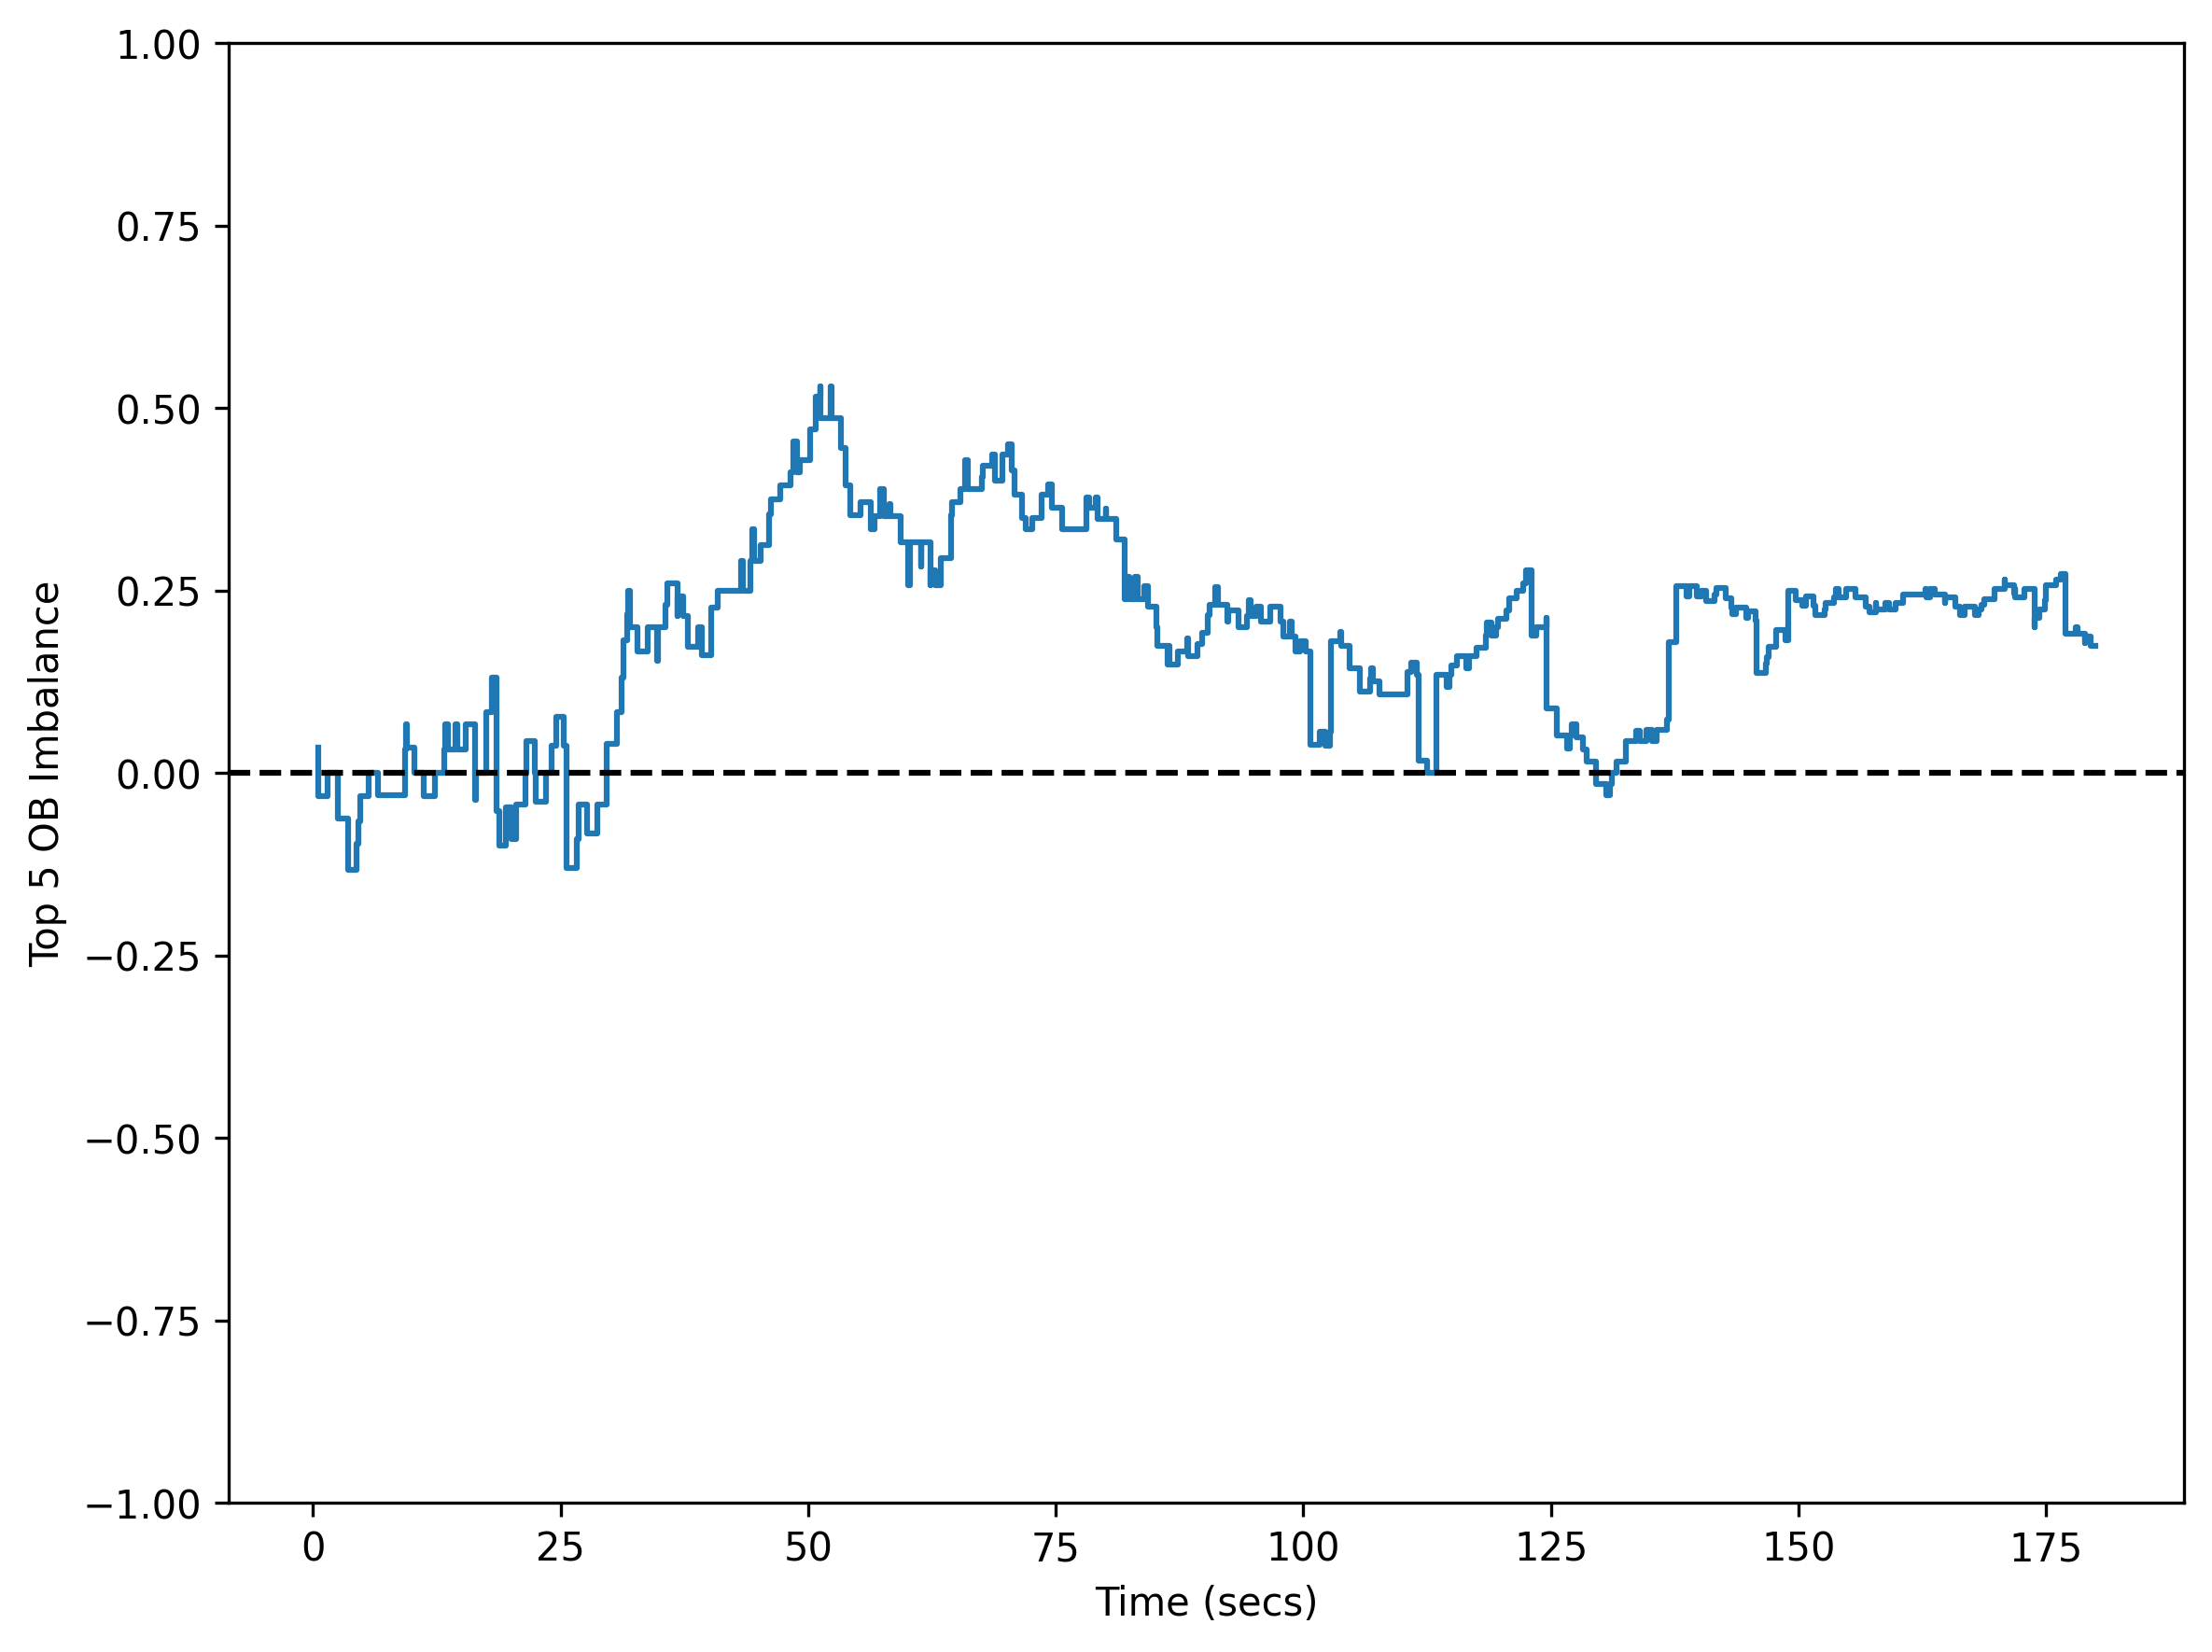
\includegraphics[scale=0.35]{figs/40_imb.png} }}
    \qquad
    \subfloat[\centering Order Flow Imbalance]{{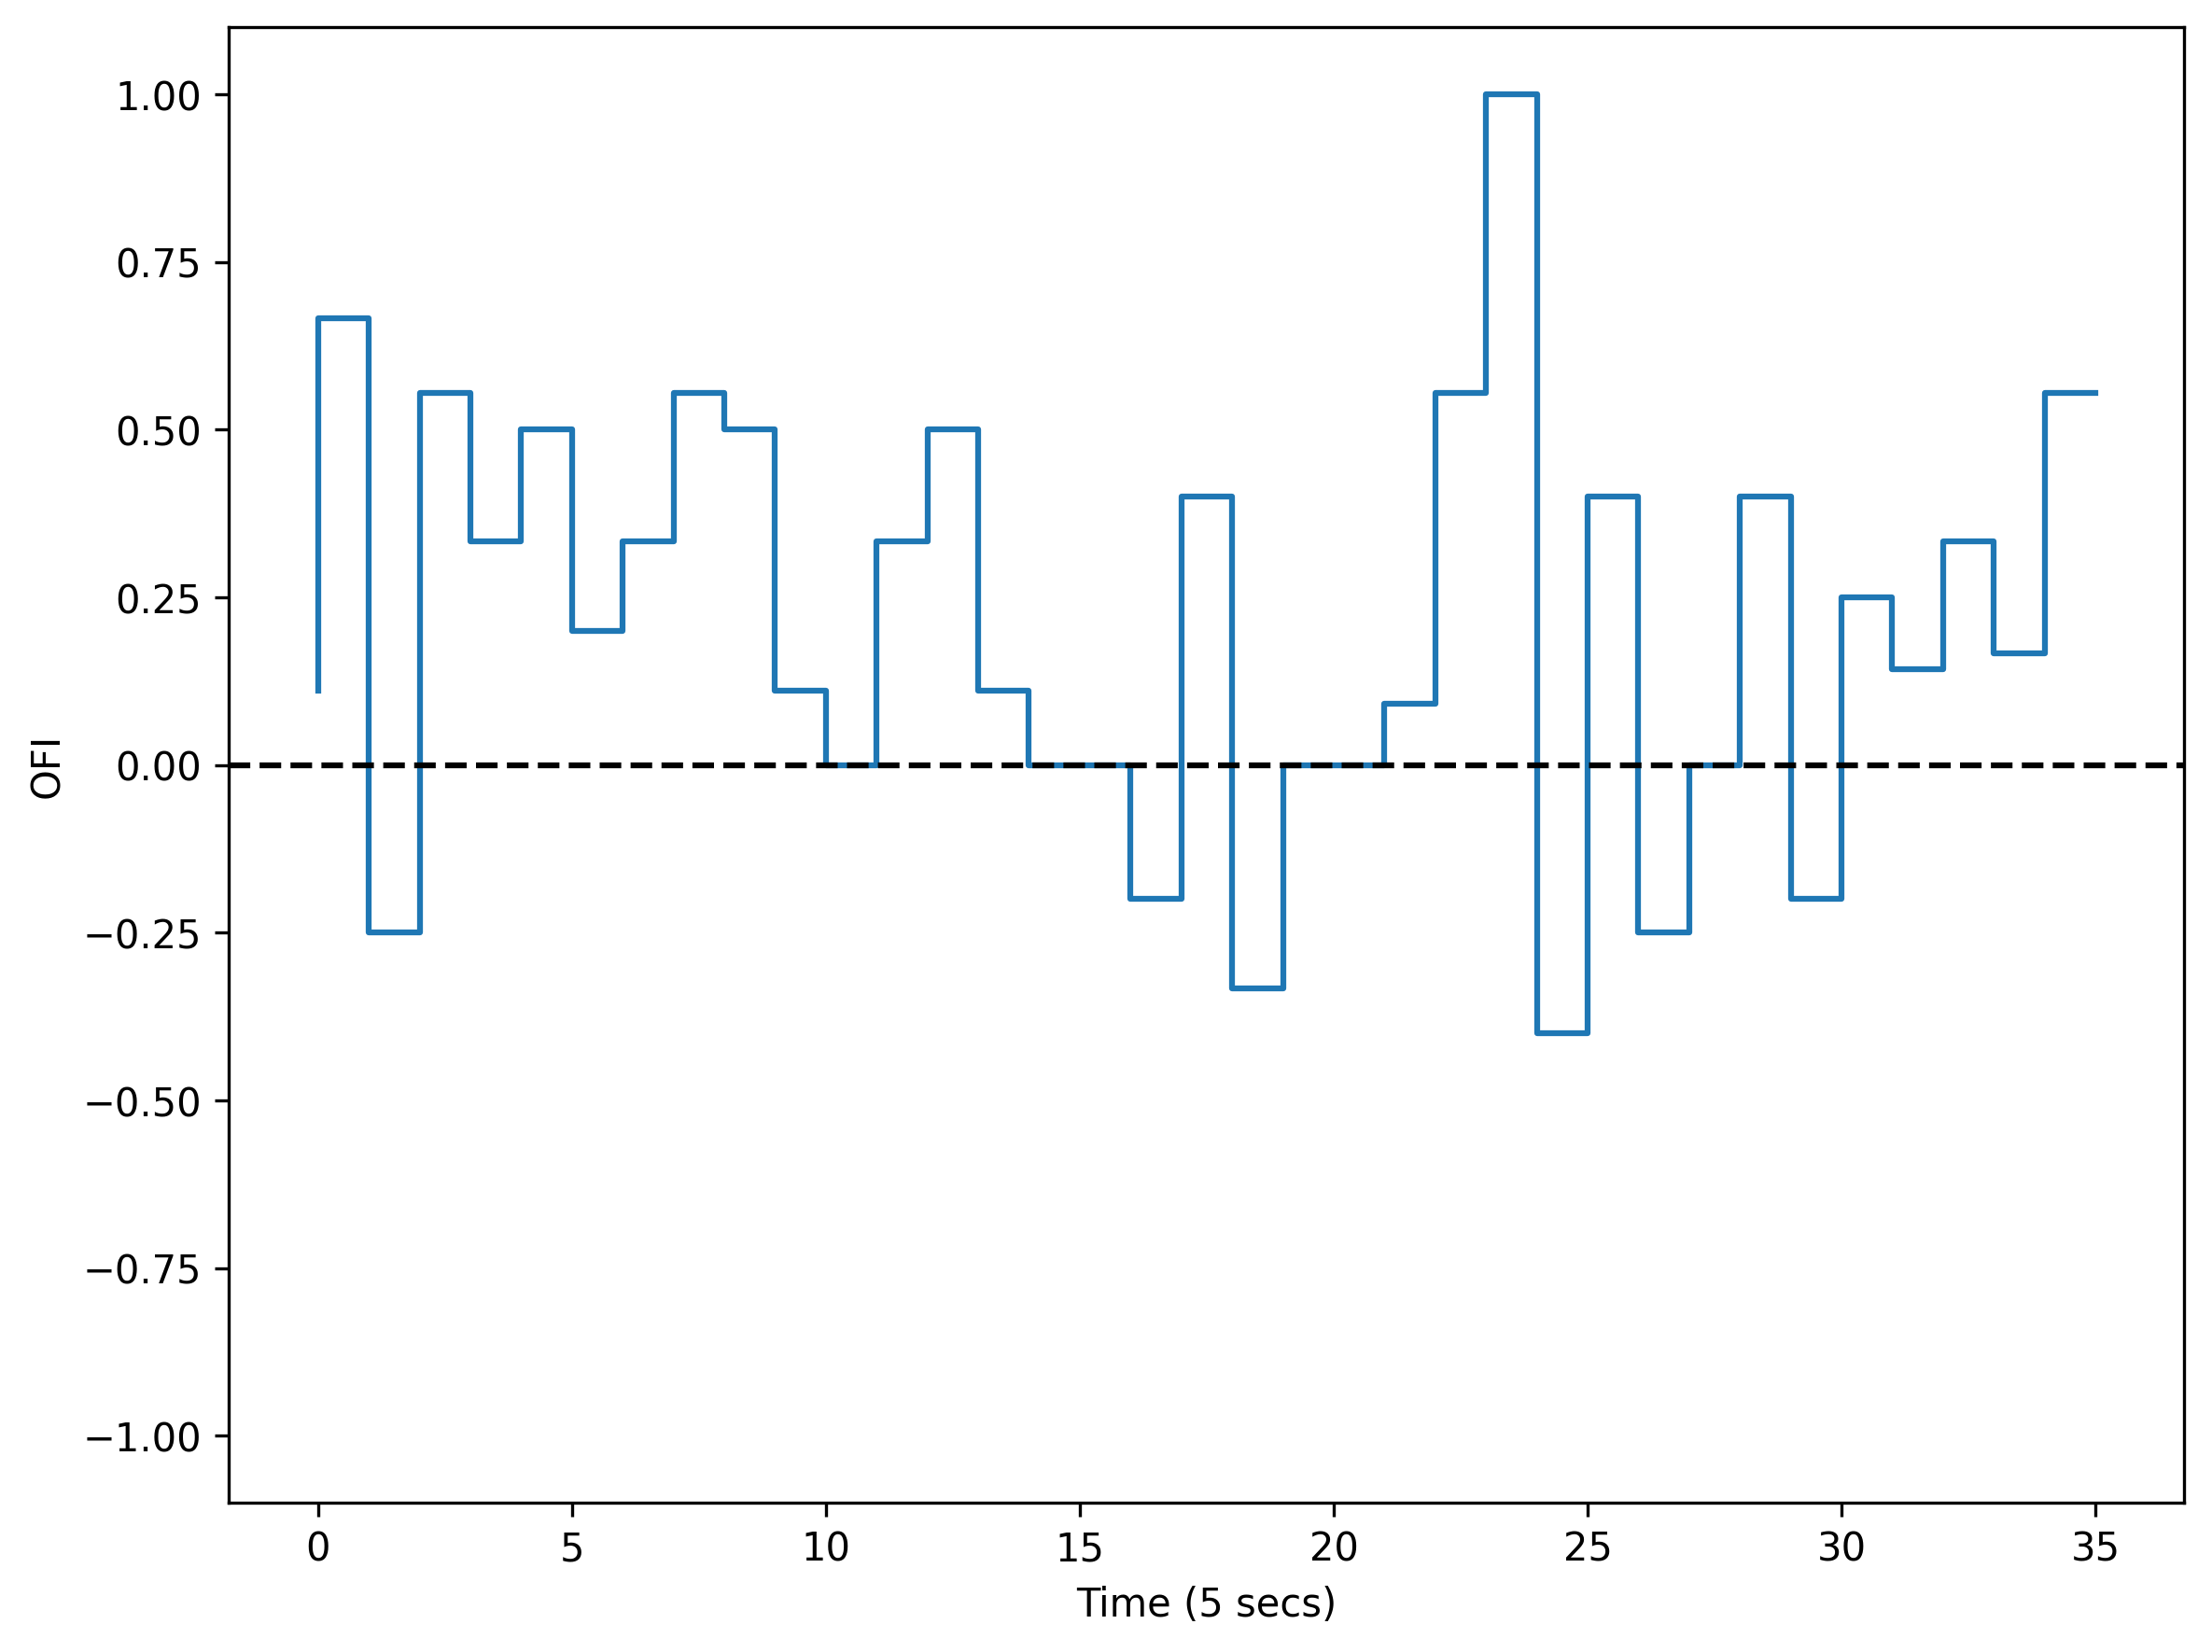
\includegraphics[scale=0.35]{figs/40_ofi.png} }}
    \qquad
    \subfloat[\centering Trade Flow Imbalance]{{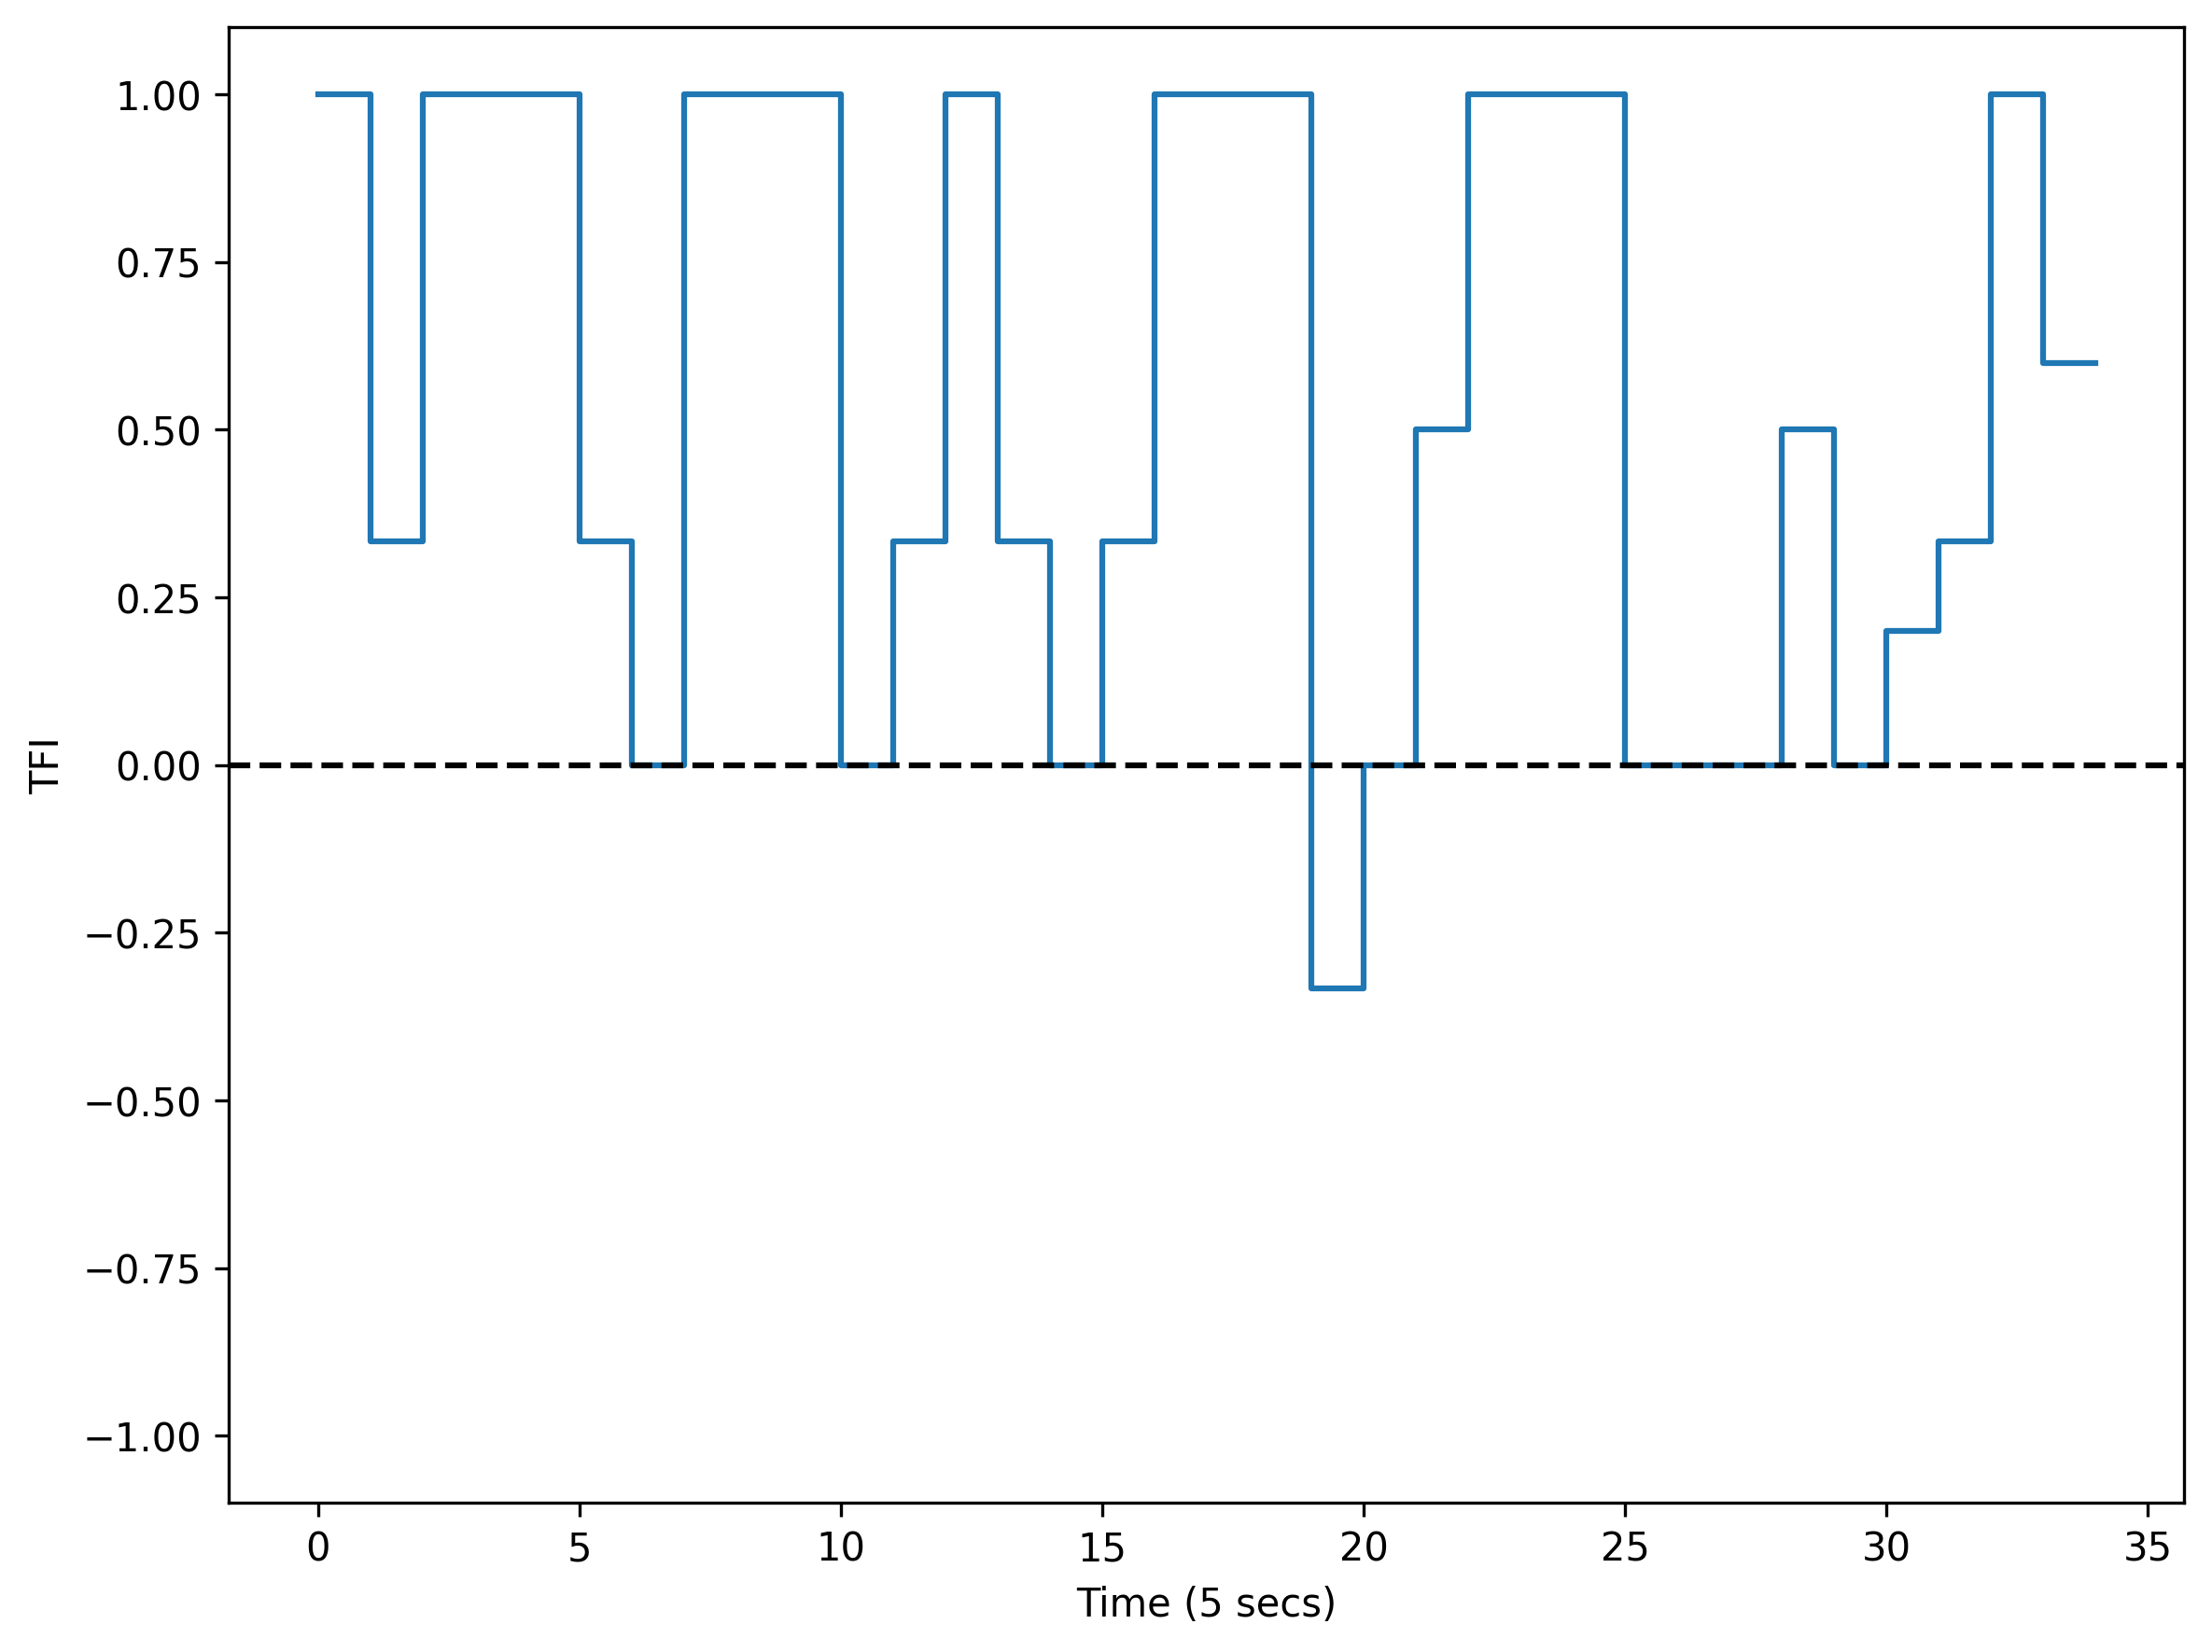
\includegraphics[scale=0.35]{figs/40_tfi.png} }}
    \caption{Additional Order Book Metrics}
    \label{fig:order_book_metrics}
\end{figure}

Figure \ref{fig:order_book_metrics} depicts the above metrics. Panel (a) illustrates the Order Book Imbalance (OBI) through the whole trading session. Panel (b) depicts the Order Flow Imbalance (OFI), and Panel (c) shows the corresponding Trade Flow Imbalance (TFI). Specifically, for OBI we used the top 5 levels, and for OFI and OBI, we aggregated the data per 5 seconds.


\section{Discussion and Future Directions}
In this section, we highlight future developments for the MINT platform, focusing on both the front-end and back-end components. The goal of these developments is to make the platform more interactive and to equip it with new tools such as the display of real time messages and the integration of GPT-assistants, which human participants could consult for trading advise. 


\subsection{Front-End}
For the front-end, we suggest including a new panel interface where participants see different messages or news in real time. This could help us study how people react to new information (positive, negative or neutral) and explore whether certain types of messages influence trading behaviour. For instance, it would be interesting to see how human trading activity evolves when neutral messages are displayed, against messages with a more positive sentiment, where a price increase is expected. While similar studies have been done using real market data (e.g. \cite{kurov2019price} among others), an experimental setup like this gives allows us to test specific causal mechanisms in a controlled and systematic environment.

Moreover, the introduction of a GPT interface would allow human participants to seek advice from different AI tools. This is quite important in practise, as would allow researchers to study the impact of AI-assisted decision-making on trading behaviour and performance, a treatment that has not been yet explored in experimental behavioural finance. 

\subsection{Backend-End}
[To be done...!]
